\section{Implementation and Evaluation Details}
\label{sec:supp_impl}
\paragraph{Family representation.}
The active encoder is a dense temporal--control mixer, not a control-wise
attention-pooling module. The observed controls are sorted by their known
coordinates before encoding. Their generated-frame latents receive a
channel-wise control embedding with width 128 and scale 0.25, and are placed
along an extended temporal axis. A learned square matrix mixes that entire
axis. VAE channels and spatial coordinates are preserved. The generated state
is one tensor with a locked reference prefix; no group of output frames is
required to equal a particular control video.

The direct query decoder uses a scalar hypernetwork with hidden width 128
and four residual blocks containing layer normalization, SiLU, and linear
layers. Its output generates a temporal weight matrix of size
$4\times J$ and a bias of size $48\times4$, where $J=36$ for lighting and
$J=12$ for MEAD. The matrix is scaled by $J^{-1/2}$ and applied to the sampled
code suffix at each channel and spatial location. The same observed reference
is prepended to every queried latent. This decoder is continuous in its scalar
input; its output need not be monotonic under an external semantic metric.

\paragraph{Optimization.}
The codec uses AdamW at learning rate $2\times10^{-4}$, zero weight decay,
and cosine decay to $2\times10^{-5}$. Training uses one complete family per
batch and 8,000 steps, with validation every 500 steps. The selected codec is
fixed before the flow model is trained. DiT adaptation uses LoRA rank 64 on
attention query, key, value, output, and two feed-forward projections, learning
rate $10^{-4}$, zero weight decay, and training seed 1234. The number of
optimizer updates is matched between LFVD and Pointwise, not the number
of processed latent tokens. Sampling uses three fixed seeds, 50 steps, and
no extra classifier-free guidance evaluation.

\paragraph{Pointwise control conditioning.}
For Lighting, the strengthened Pointwise baseline encodes $s$ as
$[s,s^2,s^3,s^4,\sin(\pi s),\cos(\pi s),\sin(2\pi s),\cos(2\pi s)]$.
Two zero-initialized projections inject this vector as a latent bias and as an
additional 4096-dimensional context token through an 8--128--4096 MLP. The
design is selected on L0 validation before the five test folds are evaluated.
It adds 529,968 parameters to the 161,218,560 LoRA parameters; the LFVD codec
has 10,493,040 parameters. On L0 validation the token changes Pointwise from
.4514 to .3917 LPIPS and raises $\rho$ from .612 to .951. Polynomial--Fourier
features were also tested in the LFVD query hypernetwork; exact-code metrics
improved slightly, but sampled metrics were unchanged (.336514 versus .336509
LPIPS and identical $\rho$). We therefore retain the scalar LFVD query.

\paragraph{LFVD-Identity protocol.}
LFVD-Identity fixes the main-paper family mixer to $\lambda=0$ and $P_\phi=I$.
It uses the same measured families, frozen VAE, Video DiT,
rank-64 LoRA targets, optimizer, update count, sampling steps, and random
seeds as LFVD-Mix. Its code is formed by directly packing the common reference
and all generated-frame latents in control order.  It removes the learned
coordinate embedding and square family mixer, but trains the same
scalar-conditioned reader with latent $L_1$ reconstruction.  The full-grid
comparison uses all measured controls during codec and flow training.  In the
sparse-control comparison, both LFVD-Identity and LFVD-Mix see only controls
$\{0,4,8\}$ and are evaluated at all nine official light positions.  Thus the
variant tests family-valued generation and learned post-hoc querying without
learned family-coordinate mixing; it is not a Pointwise sampler.
Every full-grid method is evaluated on the same locked test records in each
fold; sparse-control methods are also re-evaluated on the same locked test
records. Separate validation records agree closely.

\paragraph{Lighting coordinates.}
The nine measured controls have official light IDs
$82,81,66,64,62,61,43,60,77$, respectively. Their normalized arc coordinates
are
\begin{equation*}
\begin{split}
\{&0.0000000,0.1335363,0.2278718,\\
  &0.3818399,0.5294032,0.6233193,\\
  &0.7665081,0.9198963,1.0000000\}.
\end{split}
\end{equation*}
Each object contributes four camera windows. The five cyclic folds test
object groups 1--4, 5--8, 9--12, 13--16, and 17--20, with the next group used
for validation and the remaining three groups used for training. Each object
is tested once.

\paragraph{MEAD folds.}
The actor-disjoint test groups are (M003, M005), (M007, M009), (M011, W036),
and (W039, W040). Validation actors are M007, M011, W039, and M003,
respectively; all remaining actors form the corresponding training split.
Each actor contributes the angry and happy emotions at utterances
001, 002, 003, 007, 008, 009, and 015. The evaluated artifacts use the final
audio-DTW-aligned family release. All methods consume the same aligned
family targets and the same reference. Quantitative fidelity uses only the
three measured levels; a dense slider visualization would not add new
measured targets.

\section{Aggregate Uncertainty and Response Diagnostics}
\label{sec:supp_uncertainty}
We recompute paired intervals from the final per-family export, grouping by
object for OpenIllumination and actor for MEAD. For each metric and method,
we first average the families and three seeds within a split unit. We then
resample the 20 objects or eight actors with replacement 10,000 times and
compute the paired difference to shared-noise Pointwise. The 2.5th and
97.5th percentiles form the reported interval. This preserves within-unit
dependence and does not treat camera windows, utterances, or sampling seeds
as independent subjects. The intervals condition on the fitted checkpoints;
they do not include variation from retraining the models.

\begin{table}[t]
\centering
\caption{Paired LFVD-Mix minus shared-noise Pointwise differences. Lighting
uses the strengthened control-token Pointwise. Intervals use 10,000
object/actor-cluster resamples. Negative LPIPS and positive values for the
other metrics favor LFVD.}
\label{tab:paired_ci}
\scriptsize
\setlength{\tabcolsep}{3pt}
\begin{tabular*}{\linewidth}{@{\extracolsep{\fill}}llrc@{}}
\toprule
Dataset & Metric & Difference & 95\% interval\\
\midrule
OpenIllumination & LPIPS & -0.0414 & [-0.0511, -0.0316] \\
 & PSNR & +1.363 & [+1.139, +1.610] \\
 & SSIM & +0.0208 & [+0.0166, +0.0253] \\
 & $\rho$ & +0.0023 & [-0.0208, +0.0243] \\
\midrule
MEAD & LPIPS & -0.0006 & [-0.0151, +0.0187] \\
 & PSNR & +0.428 & [-0.086, +0.926] \\
 & SSIM & +0.0063 & [-0.0094, +0.0194] \\
 & $\rho$ & -0.0238 & [-0.1176, +0.0640] \\
\bottomrule
\end{tabular*}
\end{table}


Table~\ref{tab:paired_ci} shows a consistent Lighting improvement in LPIPS,
PSNR, and SSIM against the strengthened shared-noise Pointwise, while the
response-correlation interval includes zero. For MEAD, the intervals include
zero for all four metrics, so we report competitive mean fidelity without
asserting a statistically resolved advantage. Only eight actors contribute to
these MEAD intervals.

\begin{table}[t]
\centering
\caption{\textbf{Dense-training exposure audit} on the scene-disjoint L0
validation fold (25 steps, seed 100). Pointwise receives nine times as many
updates. This is a stress test, not the main matched-update protocol.}
\label{tab:exposure_audit}
\scriptsize
\setlength{\tabcolsep}{3.0pt}
\begin{tabular*}{\linewidth}{@{\extracolsep{\fill}}lrrrr@{}}
\toprule
Method & LPIPS$\downarrow$ & PSNR$\uparrow$ & SSIM$\uparrow$ & $\rho\uparrow$ \\
\midrule
Pointwise, $9\times$ updates & \textbf{.3268} & 20.78 & .7413 & \textbf{.9979} \\
LFVD, $1\times$ updates & .3365 & \textbf{20.86} & \textbf{.7487} & .9729 \\
\bottomrule
\end{tabular*}
\end{table}


The nine-times-update Pointwise run is evaluated only on the scene-disjoint L0
validation fold. Its update multiplier exceeds the family size and is a
deliberately strong exposure stress test, not a replacement for the locked
five-fold matched-update protocol. Pointwise wins LPIPS and ordering; LFVD
wins PSNR and SSIM. The result prevents attributing the main-table fidelity
gap solely to representation design.

\begin{table}[t]
\centering
\caption{\textbf{LFVD-Identity minus LFVD-Mix, five Lighting folds.}
Intervals use 10,000 paired bootstrap draws over 20 held-out objects. Positive
LPIPS and negative PSNR, SSIM, or $\rho$ favor LFVD-Mix.}
\label{tab:joint_concat_5fold_ci}
\scriptsize
\setlength{\tabcolsep}{3.1pt}
\begin{tabular}{llrrr}
\toprule
Protocol & Metric & Mean & 95\% CI low & 95\% CI high \\
\midrule
Full grid & LPIPS & -.0014 & -.0058 & .0030 \\
          & PSNR  & -.0043 & -.0943 & .0853 \\
          & SSIM  & -.0019 & -.0040 & .0002 \\
          & $\rho$ & -.0040 & -.0223 & .0182 \\
Sparse unseen & LPIPS & .0007 & -.0015 & .0028 \\
              & PSNR  & -.0505 & -.0998 & -.0021 \\
              & SSIM  & -.0009 & -.0021 & .0002 \\
Sparse all & $\rho$ & .0013 & -.0037 & .0069 \\
\bottomrule
\end{tabular}
\end{table}


Table~\ref{tab:joint_concat_5fold_ci} separates the general family-valued
benefit from encoder effects. Native-length full-grid and sparse test results
are unresolved overall; sparse unseen PSNR has a tiny paired advantage for
LFVD-Mix. The raw per-family and per-seed values remain in the accompanying
result package.

\begin{table}[t]
\centering
\caption{\textbf{Encoder instances on four actor-disjoint MEAD folds.}
Means cover 112 held-out families, three seeds, and 50 diffusion steps.
The final row reports LFVD-Identity minus LFVD-Mix with a 95\% paired
actor-bootstrap interval.}
\label{tab:joint_concat_mead4fold}
\scriptsize
\setlength{\tabcolsep}{2.0pt}
\resizebox{\linewidth}{!}{%
\begin{tabular}{lrrrr}
\toprule
Method & LPIPS$\downarrow$ & PSNR$\uparrow$ & SSIM$\uparrow$ & $\rho\uparrow$ \\
\midrule
Pointwise-SN & .1157 & 22.54 & .7534 & .743 \\
Endpoint interp. & .1152 & 22.91 & .7624 & \textbf{.859} \\
LFVD-Mix & .1151 & 22.97 & .7597 & .719 \\
LFVD-Identity & \textbf{.1069} & \textbf{23.16} & \textbf{.7656} & .683 \\
\midrule
$\Delta$ Identity$-$Mix
& $-.0082$ & $+.19$ & $+.0059$ & $-.036$ \\
95\% CI
& $[-.0204,-.0002]$ & $[.00,.46]$ & $[-.0003,.0158]$ & $[-.097,.018]$ \\
\bottomrule
\end{tabular}
}
\end{table}


Table~\ref{tab:joint_concat_mead4fold} provides the corresponding dynamic-video
comparison. LFVD-Identity improves mean LPIPS and PSNR over LFVD-Mix, with paired
actor-bootstrap intervals excluding zero, while SSIM and control ordering are
unresolved. This reinforces the interpretation of direct packing as a strong
family-valued encoder.

\begin{table}[t]
\centering
\caption{\textbf{Target-relative query-path consistency on Lighting.}
Errors compare each generated nine-query path with its measured target path;
lower is better. Results use 80 held-out families and seed 100.}
\label{tab:query_path}
\scriptsize
\setlength{\tabcolsep}{2.6pt}
\begin{tabular*}{\linewidth}{@{\extracolsep{\fill}}lrrr@{}}
\toprule
Method & Adj. LPIPS MAE & Path log err. & Jerk log err. \\
\midrule
Pointwise independent & .1190 & .5100 & .4712 \\
Pointwise shared      & .0867 & .5866 & .5176 \\
Endpoint interpolation & .1439 & 1.7460 & 2.1358 \\
\textbf{LFVD} & \textbf{.0303} & \textbf{.1341} & \textbf{.1588} \\
\bottomrule
\end{tabular*}
\end{table}


The target-relative path metrics use the official nine-control Lighting
targets and one common sample seed. Adjacent LPIPS error is the mean absolute
difference between generated and measured adjacent-query LPIPS. Path and jerk
errors are absolute log ratios of total adjacent LPIPS length and RMS
second-order RGB variation, respectively. Consequently, a collapsed path has
large error even if it is smooth. LFVD-minus-shared-Pointwise paired intervals
are $[-.0621,-.0506]$, $[-.5304,-.3789]$, and $[-.4489,-.2792]$ for the three
columns in Table~\ref{tab:query_path}.

\begin{table}[t]
\centering
\caption{\textbf{Reader ablation on the same sampled sparse family codes.}
The learned reader and adjacent linear interpolation receive identical LFVD-
Identity codes. Results cover five folds, three seeds, and 50 steps.}
\label{tab:reader_ablation}
\scriptsize
\setlength{\tabcolsep}{3.1pt}
\begin{tabular*}{\linewidth}{@{\extracolsep{\fill}}lrrrr@{}}
\toprule
Reader & LPIPS$\downarrow$ & PSNR$\uparrow$ & SSIM$\uparrow$ & $\rho\uparrow$ \\
\midrule
Adjacent linear & .4074 & 20.11 & .7319 & \textbf{.9918} \\
\textbf{Learned $R_\psi$} & \textbf{.3269} & \textbf{21.20} & \textbf{.7499} & .9902 \\
\bottomrule
\end{tabular*}
\end{table}


The reader ablation reuses exactly the same sampled LFVD-Identity family code
for both rows. The adjacent baseline selects the two neighboring packed latent
segments and linearly interpolates them. The learned reader improves LPIPS by
.0805 (95\% CI $[.0488,.1132]$), PSNR by 1.10 dB ($[.11,2.13]$), and SSIM by
.0180 ($[.0016,.0353]$), with nearly identical ordering.

\begin{table*}[t]
\centering
\caption{\textbf{Full sparse-control stress-test results.}
Only controls $\{0,4,8\}$ are used for training. Pointwise receives nine
times the main update budget; LFVD is the unchanged sparse model. Means cover
80 test families, three seeds, and 50 steps.}
\label{tab:sparse_control_full}
\small\setlength{\tabcolsep}{5pt}\renewcommand{\arraystretch}{1.12}
\begin{tabular*}{\textwidth}{@{\extracolsep{\fill}}lccccc c@{}}
\toprule
& \multicolumn{2}{c}{\textbf{Observed controls (3)}} & \multicolumn{2}{c}{\textbf{Unseen measured controls (6)}} & \textbf{Control} & \textbf{Updates} \\
\cmidrule(lr){2-3}\cmidrule(lr){4-5}\cmidrule(lr){6-6}\cmidrule(l){7-7}
Method & LPIPS $\downarrow$ & PSNR $\uparrow$ & LPIPS $\downarrow$ & PSNR $\uparrow$ & $\rho\uparrow$ & relative \\
\midrule
Pointwise (control token) & \textbf{0.2895} & \textbf{21.34} & \textbf{0.3322} & 20.58 & 0.9691 & $9\times$ \\
\textbf{LFVD-Mix} & 0.2993 & 20.99 & 0.3410 & \textbf{21.22} & \textbf{0.9906} & $1\times$ \\
\bottomrule
\end{tabular*}
\end{table*}


The full sparse-control export includes both observed-control metrics and the
relative update budgets. It is the same five-fold, three-seed evaluation as
the compact main-paper table; no validation families are included.

% Control sweeps decoded from one LFVD trajectory (MotionStone Fig. 5/6 style).
\begin{figure*}[t]
\centering
\qsetup{\dimexpr(\textwidth-13pt)/2-\qL-2pt\relax}%
\qpanel{%
  \qtitle{\textbf{(a) Lighting}\enspace{\color{qgray}held-out object 318}}
  \qframes
  \qrow{qorange}{\scriptsize\boldmath$s{=}0.000$}{\qimg{lighting_L3_f010_s100_m4_s00.png}}
  \qrow{qorange}{\scriptsize\boldmath$s{=}0.529$}{\qimg{lighting_L3_f010_s100_m4_s04.png}}
  \qrow{qorange}{\scriptsize\boldmath$s{=}1.000$}{\qimg{lighting_L3_f010_s100_m4_s08.png}}
}\hfill{\color{black!25}\vrule width .4pt}\hfill
\qpanel{%
  \qtitle{\textbf{(b) Lighting}\enspace{\color{qgray}held-out object 308}}
  \qframes
  \qrow{qorange}{\scriptsize\boldmath$s{=}0.000$}{\qimg{lighting_L3_f008_s100_m4_s00.png}}
  \qrow{qorange}{\scriptsize\boldmath$s{=}0.529$}{\qimg{lighting_L3_f008_s100_m4_s04.png}}
  \qrow{qorange}{\scriptsize\boldmath$s{=}1.000$}{\qimg{lighting_L3_f008_s100_m4_s08.png}}
}%
\par\vspace{-3pt}
\caption{\textbf{Continuous control from one LFVD trajectory.} In each panel,
all rows are decoded from one sampled family code at different control values
$s$ (orange); columns are temporal frames. Both panels show held-out
OpenIllumination objects at three measured light coordinates. No query
requires an additional Video DiT call.}
\label{fig:control_sweeps}
\end{figure*}


Figure~\ref{fig:control_sweeps} provides additional held-out Lighting
continua. Within each panel, every row is decoded from the same sampled family
code; only the requested physical light coordinate changes.

\section{Representation and Training-Family Scaling}
\label{sec:supp_scaling}
The completed scaling study uses nested training sets of 1, 2, 4, 8, 16, 32, and
48 lighting families and the same 16-family L0 validation split. The recorded
protocol uses 8,000 codec steps and 3,456 flow updates, a 25-step sampler,
and seed 100. The 48-family row reuses the selected full-setting evaluation.
The 32-family entry is completed in the final ablation export. These are validation analyses,
not additional held-out test results.

\begin{table}[t]
\centering
\caption{Measured lighting validation scaling rows. Exact and sampled
columns report LPIPS; the final column is sampled-code control correlation.}
\label{tab:family_scaling}
\small\setlength{\tabcolsep}{4pt}
\begin{tabular*}{\linewidth}{@{\extracolsep{\fill}}rccc@{}}
\toprule
Families & Exact $\downarrow$ & Sampled $\downarrow$ & $\rho\uparrow$\\
\midrule
1 & 0.0642 & 0.4500 & 0.4115 \\
2 & 0.0642 & 0.4409 & 0.4385 \\
4 & 0.0642 & 0.4170 & 0.7948 \\
8 & 0.0642 & 0.4021 & 0.8104 \\
16 & 0.0642 & 0.3772 & 0.9010 \\
32 & 0.0642 & 0.3450 & 0.9542 \\
48 & 0.0642 & 0.3365 & 0.9729 \\
\bottomrule
\end{tabular*}
\end{table}


\begin{figure}[t]
\centering
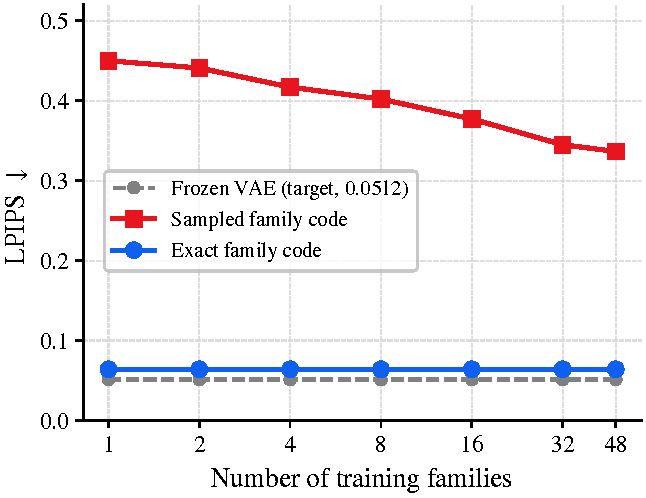
\includegraphics[width=\linewidth]{figures/family_scaling.pdf}
\caption{\textbf{Completed family-scaling study.} Exact-code reconstruction
is nearly unchanged, while sampled-code LPIPS improves as more training
families are supplied. This distinguishes family reconstruction from
conditional generation under the recorded validation protocol.}
\label{fig:family_scaling}
\end{figure}

The nearly constant exact-code result indicates that reconstruction alone
is not a reliable proxy for generative quality in this study. It does not
establish an information-theoretic capacity limit or rule out dependence on
the coordinate and training schedule. The completed coordinate comparison below shows that the retained nonlinear setting is not uniformly best across validation metrics.

\begin{figure}[t]
\centering
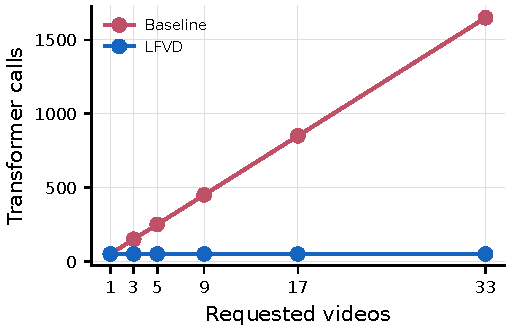
\includegraphics[width=\linewidth]{figures/call_scaling.pdf}
\caption{\textbf{Call-count scaling, not wall-clock timing.} With a fixed
50-step sampler and no classifier-free guidance branch, Pointwise uses
$50M$ transformer calls and LFVD uses 50 family-code calls. The latter
process a longer token sequence. Query and VAE costs are not represented on
this axis.}
\label{fig:call_scaling}
\end{figure}

\begin{figure*}[t]
\centering
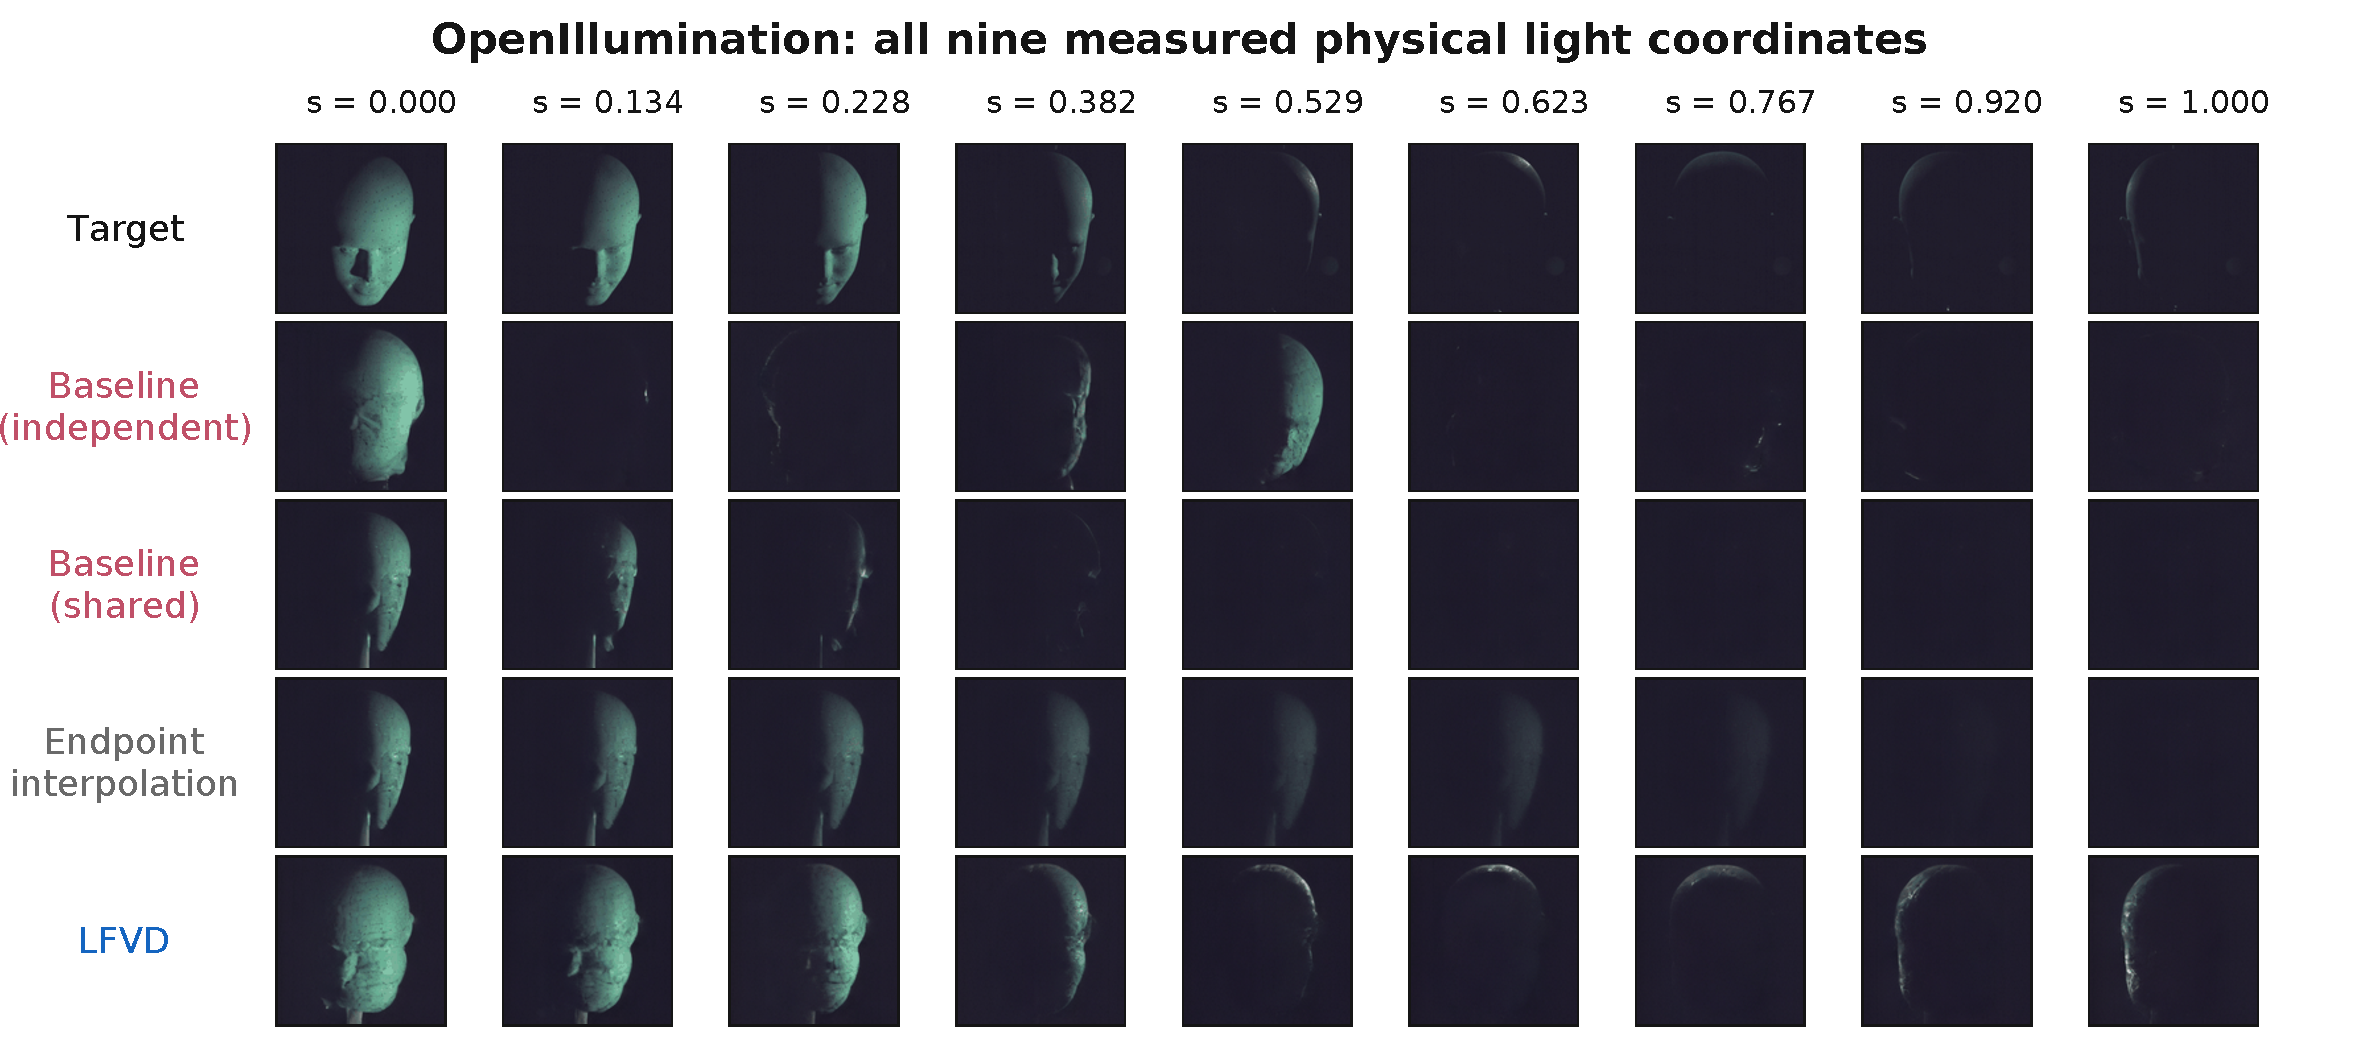
\includegraphics[width=\textwidth]{figures/fig_lighting_full.pdf}
\caption{\textbf{All measured lighting controls at one camera position.}
The fixed lighting example is the source export's median-LPIPS selection in
fold L4. Each row uses the same camera index 8. Interpolation is based on
two generated endpoints; LFVD's query is learned directly.}
\label{fig:lighting_full}
\end{figure*}

\begin{figure*}[t]
\centering
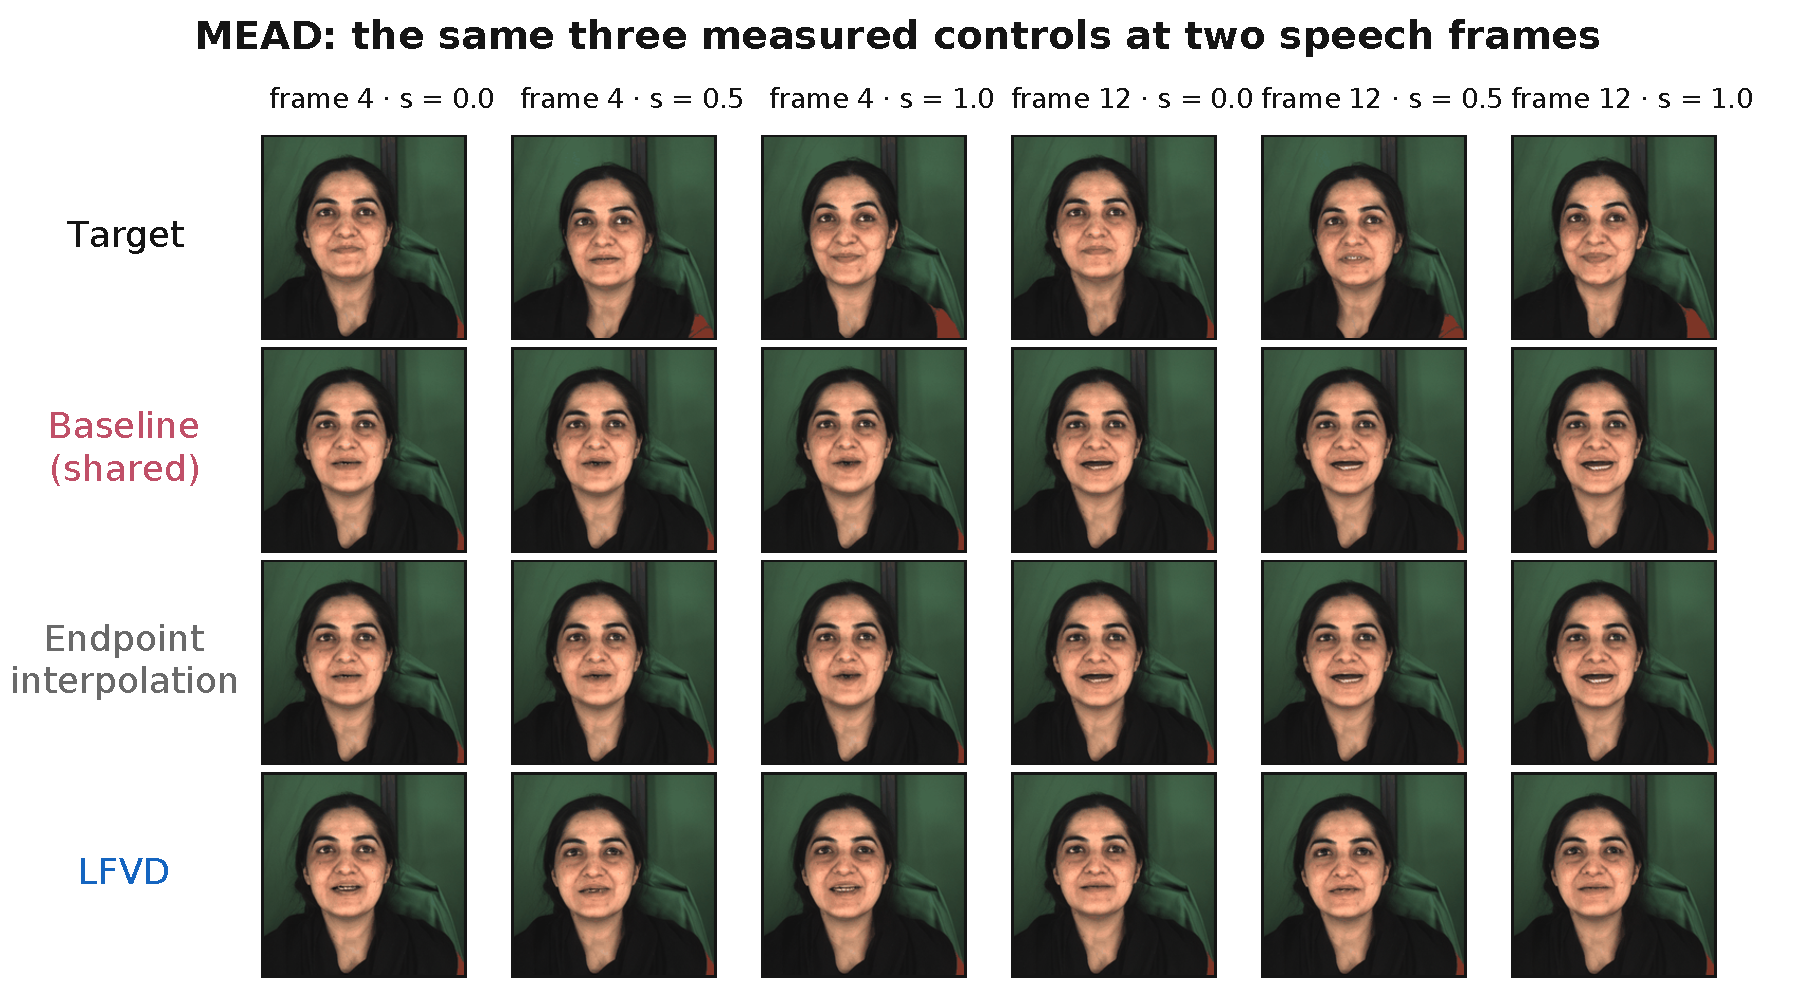
\includegraphics[width=\textwidth]{figures/fig_mead_temporal.pdf}
\caption{\textbf{Native temporal frames at measured expression levels.}
Each group of three columns shows the same actor, utterance, seed, and
speech-frame position at the three measured controls. The common reference
frame is not displayed. These crops show actual outputs and do not serve as
ground truth at an unobserved intensity.}
\label{fig:mead_temporal}
\end{figure*}


For a fixed trained family representation, increasing the number of requested
outputs does not change its denoising trajectory. The native family-code
sizes are 7.4 times (lighting) and 2.6 times (MEAD) the number of elements in
one ordinary five-frame latent, including their reference prefixes. These
ratios describe tensor sizes only.  The main paper therefore reports both
synchronized wall-clock measurements and a hardware-independent dense-matmul
count instead of converting call counts into a claimed speedup.

\paragraph{Timing protocol.}
All latency measurements use one RTX~4090, resident model weights, BF16, and
a 50-step sampler.  We synchronize CUDA immediately before and after each
timed region, discard setup and warm-up, and average three repeats.  The timed
region includes the continuous query and frozen-VAE decoding but excludes
model loading and file serialization.  Pointwise is reported sequentially
and with the strongest memory-feasible batch of three.  LFVD samples one
family code and then evaluates and decodes all requested controls.  The
reported crossover is fitted from the measured multi-query curve; it is not
inferred from trajectory counts.

\begin{figure}[t]
\centering
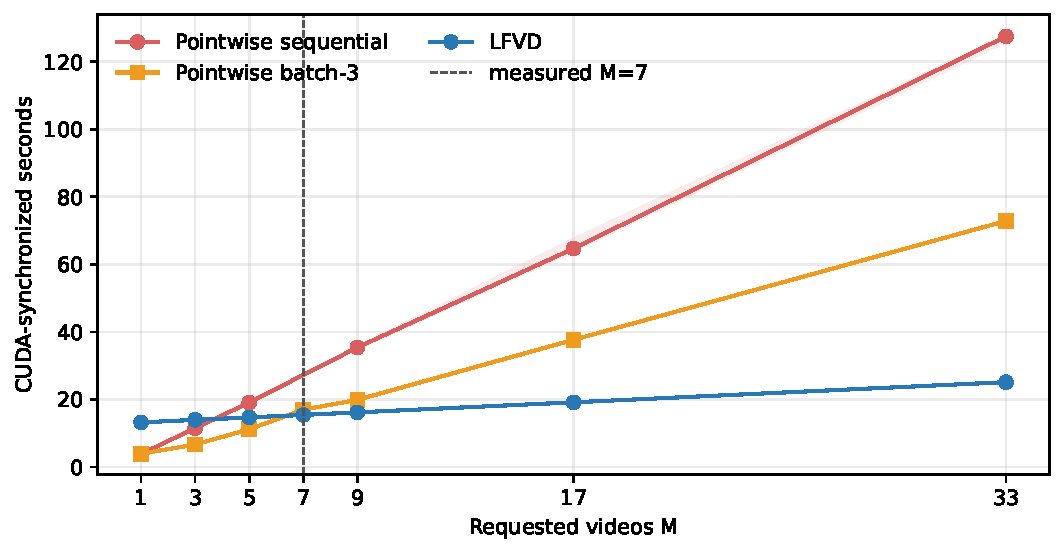
\includegraphics[width=\linewidth]{figures/reviewer_defense/lighting_cost_scaling.pdf}
\caption{\textbf{Measured inference time versus query count.} Timings use
50 denoising steps on one RTX 4090 and average three resident-model repeats.
Query and VAE decoding are included. Pointwise batch-3 is the strongest
memory-feasible batch; the measured $M=7$ point confirms the fitted crossover
at $M=6.64$.}
\label{fig:supp_measured_cost}
\end{figure}

\begin{table}[t]
\centering
\caption{Measured generation time (seconds) for $M$ requested videos,
averaged over three repeats.}
\label{tab:supp_timing}
\footnotesize
\setlength{\tabcolsep}{1.5pt}
\begin{tabular}{lrrrrrrr}
\toprule
Method & 1 & 3 & 5 & 7 & 9 & 17 & 33 \\
\midrule
Pointwise seq. & \textbf{3.88} & 11.45 & 19.06 & -- & 35.38 & 64.67 & 127.50 \\
Pointwise batch-3 & 3.90 & \textbf{6.62} & \textbf{11.16} & 16.96 & 19.86 & 37.65 & 72.84 \\
LFVD & 13.19 & 13.93 & 14.66 & \textbf{15.40} & \textbf{16.15} & \textbf{19.14} & \textbf{25.11} \\
\bottomrule
\end{tabular}
\end{table}

\paragraph{Analytical transformer work.}
The FLOP audit uses the locked Wan2.2-TI2V-5B configuration and counts dense
matrix multiplications in patch projection, 30 transformer blocks,
self-attention and cross-attention projections and attention products,
feed-forward projections, text projection, and the output head. One
multiply--accumulate is two FLOPs.  Layer normalization, elementwise
activations, the lightweight query decoder, and VAE decoding are excluded;
their device-dependent contribution is represented by the wall-clock test.
For latent lengths 5, 13, and 37, the corresponding transformer token counts
are 320, 832, and 2,368 at the recorded spatial resolution.

\begin{table}[t]
\centering
\caption{Analytical transformer cost for 50-step sampling with
Wan2.2-TI2V-5B. Query-decoder and VAE-decoder operations are excluded.}
\label{tab:supp_flops}
\footnotesize
\setlength{\tabcolsep}{4.2pt}
\begin{tabular}{lrrr}
\toprule
Representation & Latent frames & Tokens & TFLOPs/trajectory \\
\midrule
Pointwise video & 5 & 320 & 173.50 \\
MEAD family & 13 & 832 & 411.52 \\
Lighting family & 37 & 2,368 & 1,183.59 \\
\bottomrule
\end{tabular}
\end{table}

\section{Completed Lighting Ablations}
\label{sec:supp_full_ablations}
All ablations in this section use the fixed L0 lighting validation split.
The final export freezes the 3,456-update flow training schedule, a
25-step sampler, seed 100, and the same frozen VAE. The following tables
are separate from the three-seed, 50-step object-disjoint main evaluation.

\begin{table}[t]
\centering
\caption{\textbf{Coordinate sensitivity on lighting validation.} Exact-code
and sampled-code LPIPS use the same decoder. Sampling uses 25 steps and one
seed; these values are not the main test results. The main setting is retained
without claiming that it wins this sweep.}
\label{tab:coordinate_ablation}
\scriptsize
\setlength{\tabcolsep}{3.2pt}
\renewcommand{\arraystretch}{1.12}
\begin{tabular*}{\linewidth}{@{\extracolsep{\fill}}lcccc@{}}
\toprule
Coordinate & Scale & Exact $\downarrow$ & Sampled $\downarrow$ & $\rho\uparrow$\\
\midrule
None & -- & 0.0642 & 0.3351 & 0.9531 \\
Nonlinear (main) & 0.25 & 0.0642 & 0.3365 & 0.9729 \\
Nonlinear & 0.50 & 0.0642 & 0.3341 & 0.9875 \\
Nonlinear & 1.00 & 0.0642 & 0.3338 & 0.9771 \\
Linear & 0.25 & 0.0642 & 0.3242 & 0.9938 \\
\bottomrule
\end{tabular*}
\end{table}

The linear coordinate at scale 0.25 attains sampled LPIPS 0.3242 and
response $\rho=0.9938$, above the retained nonlinear scale-0.25 setting
(0.3365 and 0.9729). No claim is made that the nonlinear coordinate is
uniquely optimal. Exact-code LPIPS is nearly identical across variants.

\begin{table}[t]
\centering
\caption{\textbf{Capacity and LoRA-rank audit} (lighting L0 validation). The 24-channel code is not a runnable configuration of the fixed 48-channel direct-decoder interface; it is an architectural constraint, not a failed quality measurement.}
\label{tab:capacity_ablation}
\scriptsize\setlength{\tabcolsep}{4pt}
\begin{tabular*}{\linewidth}{@{\extracolsep{\fill}}lccc@{}}
\toprule
Variant & LPIPS $\downarrow$ & PSNR $\uparrow$ & $\rho\uparrow$ \\
\midrule
Code channels = 24 & -- & -- & -- \\
Code channels = 48 (exact) & 0.0642 & 32.06 & 1.000 \\
LoRA rank 16 (sampled) & 0.3610 & 20.60 & 0.925 \\
LoRA rank 64 (sampled) & \textbf{0.3365} & \textbf{20.86} & \textbf{0.973} \\
\bottomrule
\end{tabular*}
\end{table}

Rank-64 LoRA yields lower sampled LPIPS (0.3365) than rank-16 (0.3610)
at the recorded training budget. The narrower 24-channel family code is
not directly compatible with the frozen 48-channel query interface;
no quality metric is reported for that candidate.

\begin{table}[t]
\centering
\caption{\textbf{Representation versus generation bottleneck.} Locked lighting validation, 25-step seed-100 setting. The first row is the frozen-VAE reconstruction floor. Exact-code decoding reconstructs the observed family; the last row samples the code from conditions only.}
\label{tab:representation_bottleneck}
\scriptsize\setlength{\tabcolsep}{3pt}\renewcommand{\arraystretch}{1.12}
\begin{tabular*}{\linewidth}{@{\extracolsep{\fill}}lcccc@{}}
\toprule
Stage & LPIPS $\downarrow$ & PSNR $\uparrow$ & SSIM $\uparrow$ & $\rho\uparrow$ \\
\midrule
Frozen-VAE target & \textbf{0.0512} & \textbf{33.17} & \textbf{0.8990} & 1.000 \\
Exact family code & 0.0642 & 32.06 & 0.8927 & 1.000 \\
Sampled family code & 0.3365 & 20.86 & 0.7487 & 0.973 \\
\bottomrule
\end{tabular*}
\end{table}

Exact-code decoding reaches .0642 LPIPS and perfect ordering, close to the
frozen-VAE reconstruction floor of .0512. Sampling the same representation
raises LPIPS to .3365, localizing the principal quality loss to diffusion of
the family code rather than the query decoder.

\begin{table}[t]
\centering
\caption{\textbf{Learned-coordinate compression, exact-code oracle.} The
37-frame native coordinate has the same temporal extent as direct packing.
Shorter coordinates are trained with the same single reconstruction objective;
no perceptual or ordering term is added.}
\label{tab:coordinate_compression}
\footnotesize
\setlength{\tabcolsep}{3.5pt}
\begin{tabular}{rrrrrr}
\toprule
Code frames & Ratio & LPIPS$\downarrow$ & PSNR$\uparrow$ & SSIM$\uparrow$ & $\rho\uparrow$ \\
\midrule
37 & 1.000 & \textbf{.0642} & \textbf{32.06} & \textbf{.8927} & 1.000 \\
28 & .757 & .0814 & 30.84 & .8843 & 1.000 \\
19 & .514 & .1065 & 29.46 & .8721 & 1.000 \\
10 & .270 & .1750 & 26.45 & .8391 & .975 \\
\bottomrule
\end{tabular}
\end{table}

A non-square LFVD-Compact encoder can change the code's temporal dimension.
The 28-frame code retains exact-code LPIPS .0814 and perfect
ordering while using 75.7\% of the native 37-frame tokens. More aggressive
compression preserves order longer than texture: 19 frames still gives
$\rho=1.0$ but degrades LPIPS to .1065.  These are representation-oracle
results.  We therefore run the 28-frame candidate through the unchanged raw
flow objective and 50-step, three-seed sampler. Its sampled LPIPS is .4053,
PSNR is 21.06 dB, and control correlation is .977. On the same L0 record,
full-length LFVD-Mix reaches .3300 LPIPS, quantifying the fidelity cost of the
shorter code. Its analytical 50-step DiT
cost is 883.87 TFLOPs versus
1183.59 TFLOPs for the 37-frame representation, moving the dense-matmul
crossover against a 5-frame Pointwise trajectory from 6.82 to 5.09 queries.
These analytical counts do not replace the measured timing experiment in the
main paper.

\begin{table}[t]
\centering
\caption{\textbf{Paired sparse-control locked-test differences} (LFVD-Mix
minus shared-noise Pointwise). Intervals use 10,000 paired cluster-bootstrap
draws over 20 held-out objects.}
\label{tab:sparse_ci}
\scriptsize\setlength{\tabcolsep}{3pt}
\begin{tabular*}{\linewidth}{@{\extracolsep{\fill}}lcc@{}}
\toprule
Metric & Difference & 95\% interval \\
\midrule
Unseen LPIPS $\downarrow$ & -0.0693 & [-0.0825, -0.0576] \\
Unseen PSNR $\uparrow$ & +2.409 & [+2.127, +2.691] \\
Unseen SSIM $\uparrow$ & +0.0248 & [+0.0191, +0.0305] \\
Control $\rho\uparrow$ & +0.386 & [+0.316, +0.464] \\
\bottomrule
\end{tabular*}
\end{table}

The sparse-control stress test evaluates original measured photographs, never
interpolated or model-generated targets. Pointwise uses the frozen control
token and 31,104 updates; LFVD uses the unchanged sparse checkpoint. The mixed
LPIPS/PSNR result is therefore reported as a trade-off, not an LFVD quality
win.

\begin{figure}[t]
\centering
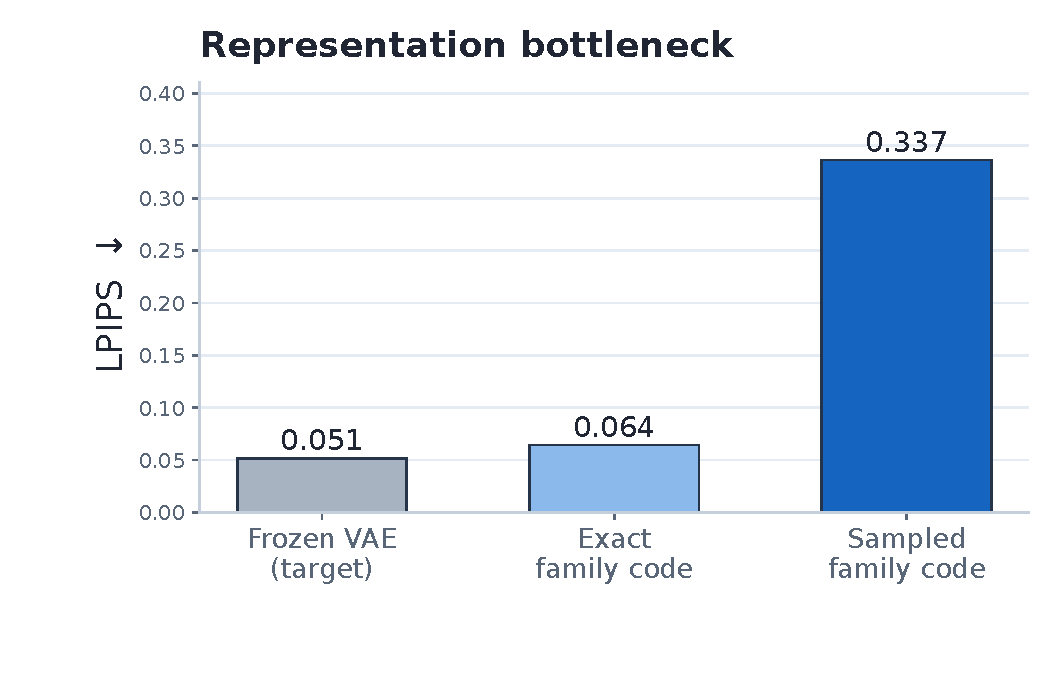
\includegraphics[width=\linewidth]{figures/fig_bottleneck_ablation.pdf}
\caption{\textbf{Bottleneck decomposition} on the locked lighting validation
fold: frozen VAE reconstruction, query from an exact family code, and
query from a DiT-sampled family code. Lower LPIPS is better; bars show
measured averages and are not bootstrap intervals.}
\label{fig:bottleneck_ablation}
\end{figure}
